\noindent
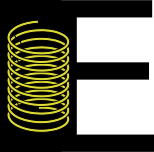
\includegraphics[height=1.25cm]{images/pictograms/elasticity}

\includegraphics[height=1.25cm]{images/pictograms/benchmark}

\includegraphics[height=1.25cm]{images/pictograms/under_construction}
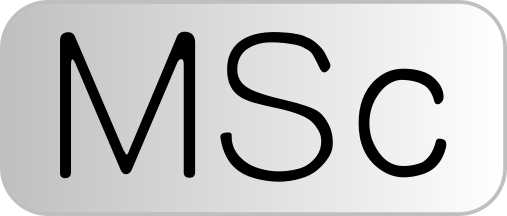
\includegraphics[height=1.25cm]{images/pictograms/msc}

\includegraphics[height=1.25cm]{images/pictograms/FEM}

\includegraphics[height=1.25cm]{images/pictograms/3d}

\includegraphics[height=1.25cm]{images/pictograms/paraview}

\includegraphics[height=1.25cm]{images/pictograms/clean}

%%%%%%%%%%%%%%%%%%%%%%%%%%%%%%%%%%%%%%%%%%%%%%%%%%%%%%%%%%%%%%%%%%%%%%%%%%%%%%%%%%%%%%%%%%%%%%%%%%%

\begin{flushright} {\tiny {\color{gray} python\_codes/fieldstone\_185/text.tex}} \end{flushright}

%\lstinputlisting[language=bash,basicstyle=\small]{python_codes/template_keywords.key}

\par\noindent\rule{\textwidth}{0.4pt}

\begin{center}
\inpython
{\small Code: \url{https://github.com/cedrict/fieldstone/tree/master/python_codes/fieldstone_185}}
\end{center}

\par\noindent\rule{\textwidth}{0.4pt}

{\sl This stone was developed in collaboration with Jacqueline Reber}. 

\par\noindent\rule{\textwidth}{0.4pt}

Last revision: June 1st, 2026.

\par\noindent\rule{\textwidth}{0.4pt}

%%%%%%%%%%%%%%%%%%%%%%%%%%%%%%%%%%%%%%%%%%%%%%%%%%%%%%%%%%%%%%%%%%%%%%%%%%%%%%%%%%%%%%%%%%%%%%%%%%%

This \stone is based on \stone~124. 
It is a proof of concept for a bigger study. The context is as follows::

\begin{itemize}
\item Email from Jacqueline (May 15th, 2026):
\begin{verbatim}
I'm reaching out to ask if you would potentially be interested in a collaboration. 
Sarah Titus (Carleton College) and I are working on a project on borehole breakouts and stress 
distribution in the crust, and we could use some numerical help. If any of this sounds vaguely 
interesting and you would potentially be up for collaborating, we could setup a call to talk 
about the project in more detail. If not, no hard feelings! I just thought it would be nice to 
work together at some point, and you came to mind instantly when we were chatting about 
modelers who would be fun to work with.
\end{verbatim} 

\item Email from Jacqueline (May 29th, 2026):
\begin{verbatim}
Input data for model on impact of layers on stress 
Dimensions of the cube: 100x100x100 mm
Dimensions of the borehole: 25 mm (diameter)
Material properties: These are approximate values for the model material. 
I would suggest we just make them a bit smaller for layer 2 
as I don’t have the actual values.
Layer 1: Youngs modulus: E = 3MPa, Shear modulus: G = 1.8 MPa
Layer 2: E = 2.5 MPa (?), G = 1 Mpa (?)
Applied stress: ~ 9kPa (sigma1). Sigma 2 and 3 can be very small.
\end{verbatim} 

Based on these values, we find the following Lam\'e's parameters

\[
\lambda_1=G_1*(E_1-2*G_1)/(3*G_1-E_1) = -450000
\qquad
\lambda_2=G_2*(E_2-2*G_2)/(3*G_2-E_2) = 1000000
\]
and the following Poisson's ratios:
\[
\nu_1=(E_1-2*G_1)/(2*G_1)= -0.1666666666
\qquad
\nu_2=(E_2-2*G_2)/(2*G_2)= 0.25
\]

A negative Poisson's ratio means a material expands perpendicular to 
a pulling force (gets wider when stretched) or compresses inward when pushed, 
directly opposite to conventional materials.
See \url{https://en.wikipedia.org/wiki/Auxetics}


\item Email from Jacqueline (June 1st, 2026):

\begin{verbatim} 
It's hard to find a value for Poisson's ratio for this experimental material. 
In light of this, can we try assuming that the poisson's ratio is similar 
to other cohesive granular materials and somewhere between 0.2-0.35? Assuming 
an E value of around 3MPa sounds reasonable to me.
\end{verbatim} 

In this case we fix $E_1=3\si{\mega\pascal}$ and assuming $\nu_1=0.3$, we obtain
\[
\lambda_1 = \frac{E \nu}{(1+\nu)(1-2\nu)} \simeq 1.73077e6
\qquad
G_1=\frac{E}{2(1+\nu)} \simeq 1.15385e6
\]

\end{itemize}



%%%%%%%%%%%%%%%%%%%%%%%%%%%%%%%%%%%%%%%%%%%%%%%%%%%%%%%%%
\section*{Meshing} 

The mesh of \stone~124 is extruded in the $z$ direction 
to produce a cuboid of size $L_x\times L_y \times L_z$ 
with a hollow cylinder in its middle:

\begin{center}
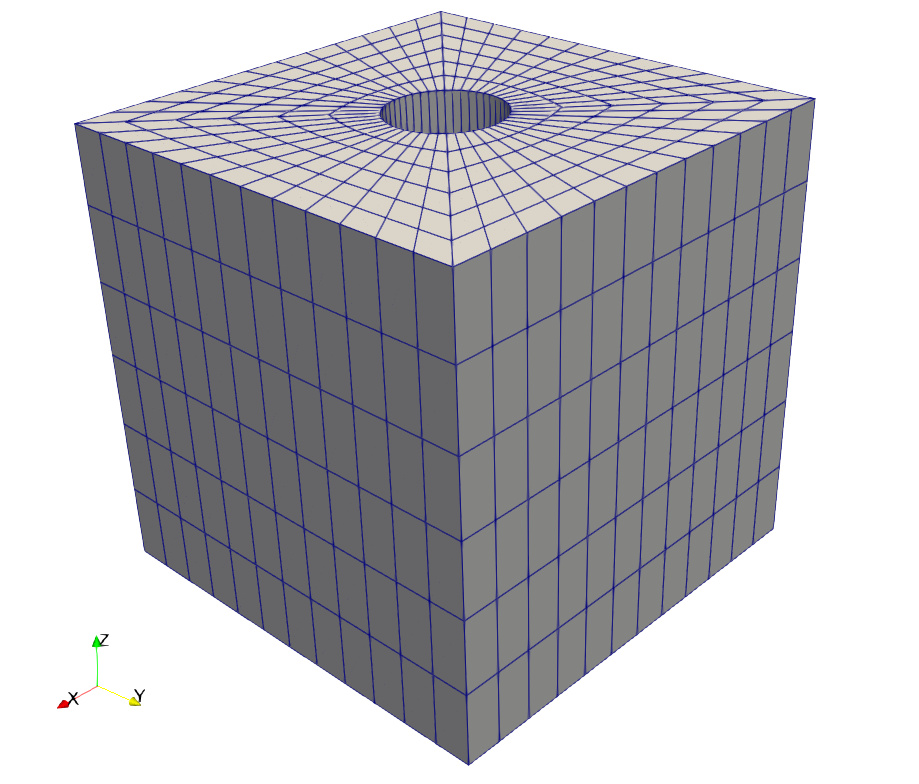
\includegraphics[width=6cm]{python_codes/fieldstone_185/images/mesh}
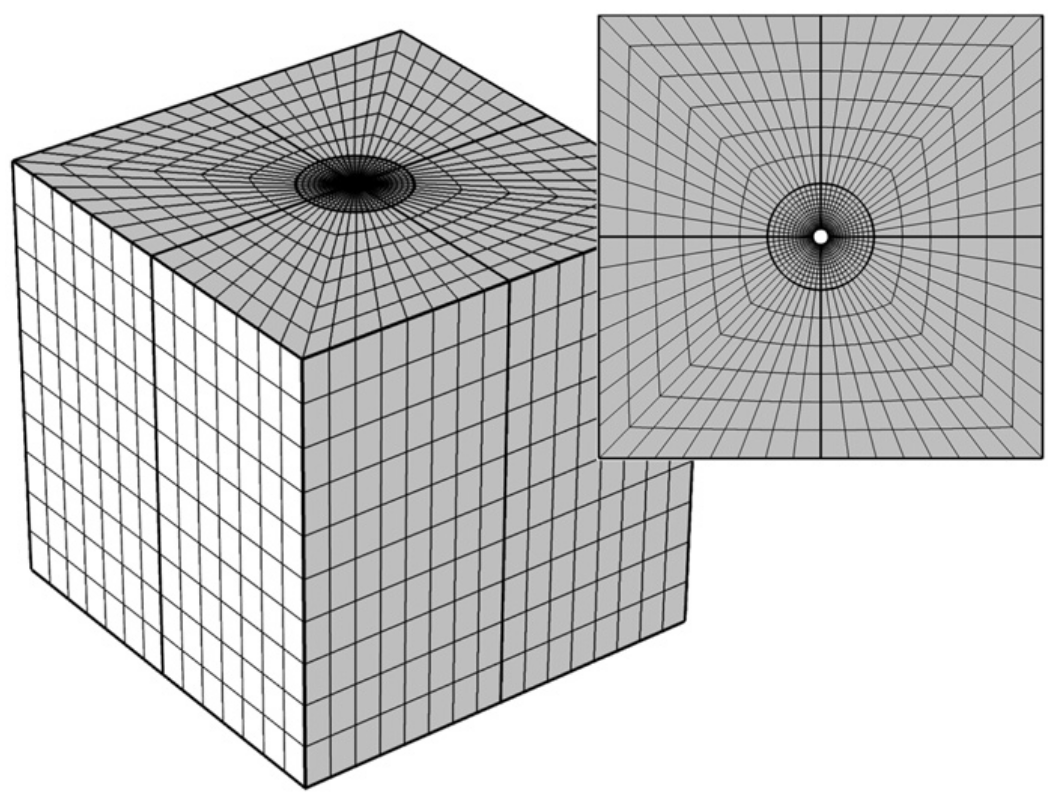
\includegraphics[width=6cm]{python_codes/fieldstone_185/images/gakj12}\\
{\captionfont Left: our mesh. Right: the mesh used in \textcite{gakj12} (2012).}
\end{center}



%%%%%%%%%%%%%%%%%%%%%%%%%%%%%%%%%%%%%%%%%%%%%%%%%%%%%%%%%
\section*{Numerical methods}

We here use the FEM to solve the mechanical equilibrium equations in 3d.
Quadrilateral linear elements ($Q_1$) are used.
The theory and implementation details of linear elasticity
are presented in Section~\ref{MMM-chapt:elasticity}.

Very briefly:
\begin{equation}
\underbrace{
\left( \begin{array}{c}
\sigma_{xx} \\
\sigma_{yy} \\
\sigma_{zz} \\
\sigma_{xy} \\
\sigma_{xz} \\
\sigma_{yz} 
\end{array} \right)}
_{\vec{\sigma}}
=
\underbrace{
\left( \begin{array}{cccccc}
\lambda+2\mu & \lambda & \lambda & 0 & 0 & 0 \\ 
\lambda & \lambda+2\mu & \lambda & 0 & 0 & 0 \\ 
\lambda & \lambda & \lambda+2\mu & 0 & 0 & 0 \\
0 & 0 & 0 & \mu & 0 & 0 \\ 
0 & 0 & 0 & 0 & \mu & 0 \\ 
0 & 0 & 0 & 0 & 0 & \mu  
\end{array} \right)}
_{{\bm C}}
\cdot
\underbrace{
\left( \begin{array}{c}
\varepsilon_{xx} \\
\varepsilon_{yy} \\
\varepsilon_{zz} \\
{\color{teal}2}\varepsilon_{xy} \\
{\color{teal}2}\varepsilon_{xz} \\
{\color{teal}2}\varepsilon_{yz} 
\end{array} \right)}
_{\vec{\varepsilon}}
\label{eq:el:vectors}
\end{equation}

The incompressibility (or bulk modulus) $K$ is defined as 
$p=-K \vec{\nabla}\cdot\vec{\upupsilon}$ where $p$ is the pressure with 
\begin{eqnarray}
p &=& -\left( \lambda + \frac{2}{3} \mu \right) (\vec{\nabla}\cdot\vec{\upupsilon})  
\end{eqnarray}

finally the deviatoric stress ${\bm \tau}$ is given by:
\[
\vec{\tau}=
\left( \begin{array}{cccccc}
\frac23 & - \frac13 & - \frac13 & 0 & 0 & 0 \\
-\frac13 & \frac23 & - \frac13  & 0 & 0 & 0\\
-\frac13& - \frac13 & \frac23  & 0 & 0 & 0\\
0&0&0& 1&0 &0  \\
0&0&0&0&1 &0\\
0&0&0&0&0& 1
\end{array} \right)
\cdot
\left( \begin{array}{c}
\sigma_{xx}\\
\sigma_{yy}\\
\sigma_{zz}\\
\sigma_{xy}\\
\sigma_{xz}\\
\sigma_{yz}
\end{array} \right)
\]





Each element is assigned a Young's modulus value $E$ and a 
shear modulus value $G$ so that the matrix ${\bm C}$ can be built.

Boundary conditions are a mix of Dirichlet and Neumann ones.
A traction $\sigma_{bc}$ is applied to the faces $x=0$ and $x=L_x$.
As such boundary conditions result in 3 translational nullspaces
a zero tangential velocity is prescribed in the middle of all 
four vertical faces.


%%%%%%%%%%%%%%%%%%%%%%%%%%%%%%%%%%%%%%%%%%%%%%%%%%%%%%%%%
\section*{to do ...}

carry out analytical bench a la f124

make oval hole ?

deform borehole

add stress bc in other direction 

compute principal stresses

%%%%%%%%%%%%%%%%%%%%%%%%%%%%%%%%%%%%%%%%%%%%%%%%%%%%%%%%%

 



